\newpage
\null
\thispagestyle{empty}
\newpage

\addcontentsline{toc}{chapter}{Romans}
% Safely inserts your illustration full-bleed on its own page.
% This completely bypasses the page builder, headers, and geometry bugs!
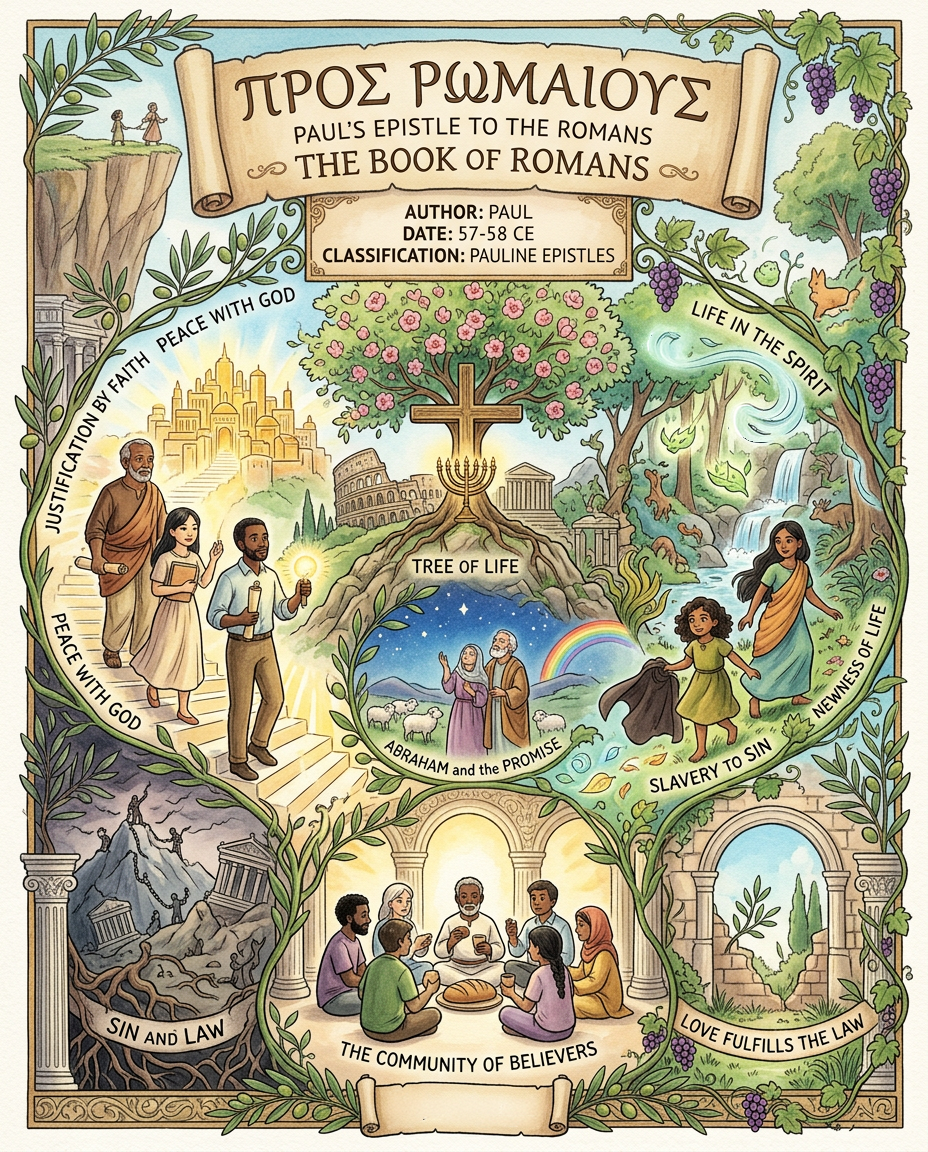
\includepdf[pages=1, fitpaper=false, width=\paperwidth, height=\paperheight, , keepaspectratio=false]{images/divider2/romans2.png}
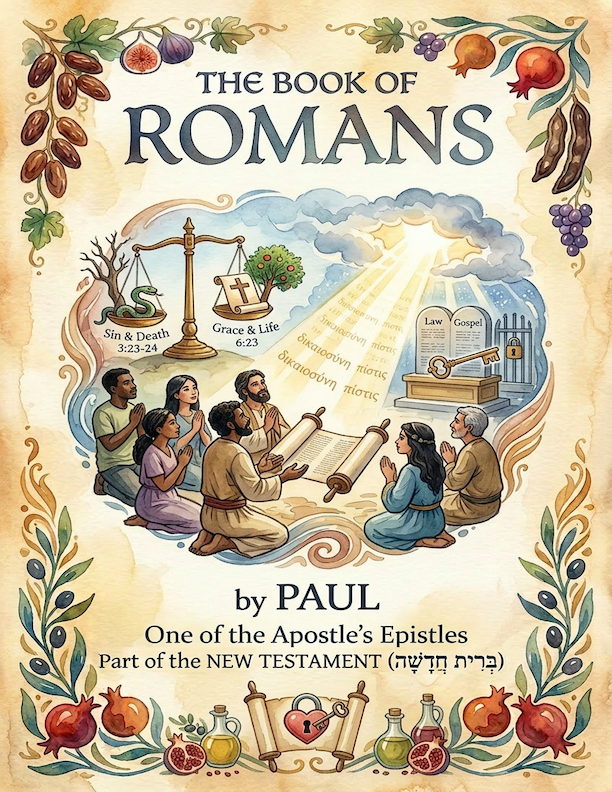
\includepdf[pages=1, fitpaper=false, width=\paperwidth, height=\paperheight, , keepaspectratio=false]{images/divider1/romans.png}

\includepdf[pages=1, fitpaper=false, width=\paperwidth, height=\paperheight, , keepaspectratio=false]{images/8.5x11-Dot-Grid.png}

\includepdf[pages=1, fitpaper=false, width=\paperwidth, height=\paperheight, , keepaspectratio=false]{images/8.5x11-Dot-Grid.png}
\mybook{Romans}
\vspace{-1.36in}


\mychapter{} \myverse*{}Paul, a servant of Yeshua the Messiah,\footnote{1:1 “Messiah” means “Anointed One”.} called to be an emissary, set apart for the Good News
of God,
\myverse{}which he promised before through his prophets in the holy Scriptures,
\myverse{}concerning his Son, who was born of the offspring\footnote{1:3 or, seed} of David according to the flesh,
\myverse{}who was declared to be the Son of God with power according to the Spirit of
holiness, by the resurrection from the dead, Yeshua the Messiah our Lord,
\myverse{}through whom we received grace and the office of emissary for obedience of faith
among all the nations for his name’s sake;
\myverse{}among whom you are also called to belong to Yeshua the Messiah;
\myverse{}to all who are in Rome, beloved of God, called to be holy ones: Grace to you
and peace from God our Father and the Lord Yeshua the Messiah.

\myverse{}First, I thank my God through Yeshua the Messiah for all of you,
that your faith is proclaimed throughout the whole world.
\myverse{}For God is my witness, whom I serve in my spirit in the Good News of his Son,
how unceasingly I make mention of you always in my prayers,
\myverse{}requesting, if by any means now at last I may be prospered by the will of
God to come to you.
\myverse{}For I long to see you, that I may impart to you some spiritual gift, to the
end that you may be established;
\myverse{}that is, that I with you may be encouraged in you, each of us by the other’s
faith, both yours and mine.

\myverse{}Now I don’t desire to have you unaware, brothers, that I often
planned to come to you (and was hindered so far), that I might have some fruit among you also, even as
among the rest of the Gentiles.
\myverse{}I am debtor both to Greeks and to foreigners, both to the wise and to the
foolish.
\myverse{}So as much as is in me, I am eager to proclaim the Good News to you also who
are in Rome.

\myverse{}For I am not ashamed of the Good News of Messiah, because it
is the power of God for salvation for everyone who believes, for the Jew first, and also for the Greek.
\myverse{}For in it is revealed God’s righteousness from faith to faith. As it is written,
“But the righteous shall live by faith.”\footnote{1:17 Habakkuk 2:4}

\myverse{}For the wrath of God is revealed from heaven against all ungodliness
and unrighteousness of men who suppress the truth in unrighteousness,
\myverse{}because that which is known of God is revealed in them, for God revealed it
to them.
\myverse{}For the invisible things of him since the creation of the world are clearly
seen, being perceived through the things that are made, even his everlasting power and divinity, that
they may be without excuse.
\myverse{}Because knowing God, they didn’t glorify him as God, and didn’t give thanks,
but became vain in their reasoning, and their senseless heart was darkened.

\myverse{}Professing themselves to be wise, they became fools,
\myverse{}and traded the glory of the incorruptible God for the likeness of an image
of corruptible man, and of birds, four-footed animals, and creeping things.
\myverse{}Therefore God also gave them up in the lusts of their hearts to uncleanness,
that their bodies should be dishonored among themselves;
\myverse{}who exchanged the truth of God for a lie, and worshiped and served the creature
rather than the Creator, who is blessed forever. Amen.

\myverse{}For this reason, God gave them up to vile passions. For their
women changed the natural function into that which is against nature.
\myverse{}Likewise also the men, leaving the natural function of the woman, burned in
their lust toward one another, men doing what is inappropriate with men, and receiving in themselves the
due penalty of their error.
\myverse{}Even as they refused to have God in their knowledge, God gave them up to a
reprobate mind, to do those things which are not fitting;
\myverse{}being filled with all unrighteousness, sexual immorality, wickedness, covetousness,
malice; full of envy, murder, strife, deceit, evil habits, secret slanderers,
\myverse{}backbiters, hateful to God, insolent, arrogant, boastful, inventors of evil
things, disobedient to parents,
\myverse{}without understanding, covenant breakers, without natural affection, unforgiving,
unmerciful;
\myverse{}who, knowing the ordinance of God, that those who practice such things are
worthy of death, not only do the same, but also approve of those who practice them.


% ROMANS 2
\mychapter{} \myverse*{}Therefore you are without excuse, O man, whoever you are who judge.
For in that which you judge another, you condemn yourself. For you who judge practice the same things.
\myverse{}We know that the judgment of God is according to truth against those who practice
such things.
\myverse{}Do you think this, O man who judges those who practice such things, and do the
same, that you will escape the judgment of God?
\myverse{}Or do you despise the riches of his goodness, forbearance, and patience, not
knowing that the goodness of God leads you to repentance?
\myverse{}But according to your hardness and unrepentant heart you are treasuring up for
yourself wrath in the day of wrath, revelation, and of the righteous judgment of God,
\myverse{}who “will pay back to everyone according to their works:”\footnote{2:6 Psalms 62:12;
	Proverbs 24:12}
\myverse{}to those who by perseverance in well-doing seek for glory, honor, and incorruptibility,
eternal life;
\myverse{}but to those who are self-seeking and don’t obey the truth, but obey unrighteousness,
will be wrath, indignation,
\myverse{}oppression, and anguish on every soul of man who does evil, to the Jew first,
and also to the Greek.

\myverse{}But glory, honor, and peace go to every man who does good, to
the Jew first, and also to the Greek.
\myverse{}For there is no partiality with God.
\myverse{}For as many as have sinned without the law will also perish without the law.
As many as have sinned under the law will be judged by the law.
\myverse{}For it isn’t the hearers of the law who are righteous before God, but the
doers of the law will be justified
\myverse{}(for when Gentiles who don’t have the law do by nature the things of the law,
these, not having the law, are a law to themselves,
\myverse{}in that they show the work of the law written in their hearts, their conscience
testifying with them, and their thoughts among themselves accusing or else excusing them)
\myverse{}in the day when God will judge the secrets of men, according to my Good News,
by Yeshua the Messiah.

\myverse{}Indeed you bear the name of a Jew, rest on the law, glory in
God,
\myverse{}know his will, and approve the things that are excellent, being instructed
out of the law,
\myverse{}and are confident that you yourself are a guide of the blind, a light to those
who are in darkness,
\myverse{}a corrector of the foolish, a teacher of babies, having in the law the form
of knowledge and of the truth.
\myverse{}You therefore who teach another, don’t you teach yourself? You who proclaim
that a man shouldn’t steal, do you steal?
\myverse{}You who say a man shouldn’t commit adultery, do you commit adultery? You who
abhor idols, do you rob temples?
\myverse{}You who glory in the law, do you dishonor God by disobeying the law?
\myverse{}For “the name of God is blasphemed among the Gentiles because of you,”\footnote{2:24 Isaiah 52:5;
	Ezekiel 36:22} just as it is written.
\myverse{}For circumcision indeed profits, if you are a doer of the law, but if you
are a transgressor of the law, your circumcision has become uncircumcision.
\myverse{}If therefore the uncircumcised keep the ordinances of the law, won’t his uncircumcision
be accounted as circumcision?
\myverse{}Won’t those who are physically uncircumcised, but fulfill the law, judge you,
who with the letter and circumcision are a transgressor of the law?
\myverse{}For he is not a Jew who is one outwardly, neither is that circumcision which
is outward in the flesh;
\myverse{}but he is a Jew who is one inwardly, and circumcision is that of the heart,
in the spirit, not in the letter; whose praise is not from men, but from God.


% ROMANS 3
\mychapter{} \myverse*{}Then what advantage does the Jew have? Or what is the profit of
circumcision?
\myverse{}Much in every way! Because first of all, they were entrusted with the revelations
of God.
\myverse{}For what if some were without faith? Will their lack of faith nullify the faithfulness
of God?
\myverse{}May it never be! Yes, let God be found true, but every man a liar. As it is
written,

“that you might be justified in your words,

and might prevail when you come into judgment.”\footnote{3:4 Psalms 51:4}

\myverse{}But if our unrighteousness commends the righteousness of God, what
will we say? Is God unrighteous who inflicts wrath? I speak like men do.
\myverse{}May it never be! For then how will God judge the world?
\myverse{}For if the truth of God through my lie abounded to his glory, why am I also
still judged as a sinner?
\myverse{}Why not (as we are slanderously reported, and as some affirm that we say), “Let’s
do evil, that good may come?” Those who say so are justly condemned.

\myverse{}What then? Are we better than they? No, in no way. For we previously
warned both Jews and Greeks that they are all under sin.
\myverse{}As it is written,

“There is no one righteous;

no, not one.

\myverse{}There is no one who understands.

There is no one who seeks after God.

\myverse{}They have all turned away.

They have together become unprofitable.

There is no one who does good,

no, not so much as one.”\footnote{3:12 Psalms 14:1-3;
	53:1-3;
	Ecclesiastes 7:20}

\myverse{}“Their throat is an open tomb.

With their tongues they have used deceit.”\footnote{3:13 Psalms 5:9}

“The poison of vipers is under their lips.”\footnote{3:13 Psalms 140:3}

\myverse{}“Their mouth is full of cursing and bitterness.”\footnote{3:14 Psalms 10:7}

\myverse{}“Their feet are swift to shed blood.

\myverse{}Destruction and misery are in their ways.

\myverse{}The way of peace, they haven’t known.”\footnote{3:17 Isaiah 59:7-8}

\myverse{}“There is no fear of God before their eyes.”\footnote{3:18 Psalms 36:1}

\myverse{}Now we know that whatever things the law says, it speaks to those
who are under the law, that every mouth may be closed, and all the world may be brought under the judgment
of God.
\myverse{}Because by the works of the law, no flesh will be justified in his sight;
for through the law comes the knowledge of sin.

\myverse{}But now apart from the law, a righteousness of God has been revealed,
being testified by the Torah and the Prophets;
\myverse{}even the righteousness of God through faith in Yeshua the Messiah to all and
on all those who believe. For there is no distinction,
\myverse{}for all have sinned, and fall short of the glory of God;
\myverse{}being justified freely by his grace through the redemption that is in Messiah
Yeshua,
\myverse{}whom God sent to be an atoning sacrifice\footnote{3:25 or, a propitiation} through faith in his blood, for a demonstration of his righteousness
through the passing over of prior sins, in God’s forbearance;
\myverse{}to demonstrate his righteousness at this present time, that he might himself
be just and the justifier of him who has faith in Yeshua.

\myverse{}Where then is the boasting? It is excluded. By what kind of law?
Of works? No, but by a law of faith.
\myverse{}We maintain therefore that a man is justified by faith apart from the works
of the law.
\myverse{}Or is God the God of Jews only? Isn’t he the God of Gentiles also? Yes, of
Gentiles also,
\myverse{}since indeed there is one God who will justify the circumcised by faith and
the uncircumcised through faith.

\myverse{}Do we then nullify the law through faith? May it never be! No,
we establish the law.


% ROMANS 4
\mychapter{} \myverse*{}What then will we say that Abraham, our forefather, has found according
to the flesh?
\myverse{}For if Abraham was justified by works, he has something to boast about, but
not toward God.
\myverse{}For what does the Scripture say? “Abraham believed God, and it was accounted
to him for righteousness.”\footnote{4:3 Genesis 15:6}
\myverse{}Now to him who works, the reward is not counted as grace, but as something owed.
\myverse{}But to him who doesn’t work, but believes in him who justifies the ungodly,
his faith is accounted for righteousness.
\myverse{}Even as David also pronounces blessing on the man to whom God counts righteousness
apart from works:

\myverse{}“Blessed are they whose iniquities are forgiven,

whose sins are covered.

\myverse{}Blessed is the man whom the Lord will by no means charge with
sin.”\footnote{4:8 Psalms 32:1-2}

\myverse{}Is this blessing then pronounced only on the circumcised, or on
the uncircumcised also? For we say that faith was accounted to Abraham for righteousness.
\myverse{}How then was it counted? When he was in circumcision, or in uncircumcision?
Not in circumcision, but in uncircumcision.
\myverse{}He received the sign of circumcision, a seal of the righteousness of the faith
which he had while he was in uncircumcision, that he might be the father of all those who believe, though
they might be in uncircumcision, that righteousness might also be accounted to them.
\myverse{}He is the father of circumcision to those who not only are of the circumcision,
but who also walk in the steps of that faith of our father Abraham, which he had in uncircumcision.

\myverse{}For the promise to Abraham and to his offspring that he would
be heir of the world wasn’t through the law, but through the righteousness of faith.
\myverse{}For if those who are of the law are heirs, faith is made void, and the promise
is made of no effect.
\myverse{}For the law produces wrath; for where there is no law, neither is there disobedience.

\myverse{}For this cause it is of faith, that it may be according to grace,
to the end that the promise may be sure to all the offspring, not to that only which is of the law, but
to that also which is of the faith of Abraham, who is the father of us all.
\myverse{}As it is written, “I have made you a father of many nations.”\footnote{4:17 Genesis 17:5} This is in the presence of him whom he believed:
God, who gives life to the dead, and calls the things that are not, as though they were.
\myverse{}Against hope, Abraham in hope believed, to the end that he might become a
father of many nations, according to that which had been spoken, “So will your offspring be.”\footnote{4:18 Genesis 15:5}
\myverse{}Without being weakened in faith, he didn’t consider his own body, already
having been worn out, (he being about a hundred years old), and the deadness of Sarah’s womb.
\myverse{}Yet, looking to the promise of God, he didn’t waver through unbelief, but
grew strong through faith, giving glory to God,
\myverse{}and being fully assured that what he had promised, he was also able to perform.
\myverse{}Therefore it also was “credited to him for righteousness.”\footnote{4:22 Genesis 15:6}
\myverse{}Now it was not written that it was accounted to him for his sake alone,
\myverse{}but for our sake also, to whom it will be accounted, who believe in him who
raised Yeshua our Lord from the dead,
\myverse{}who was delivered up for our trespasses, and was raised for our justification.


% ROMANS 5
\mychapter{} \myverse*{}Being therefore justified by faith, we have peace with God through
our Lord Yeshua the Messiah;
\myverse{}through whom we also have our access by faith into this grace in which we stand.
We rejoice in hope of the glory of God.
\myverse{}Not only this, but we also rejoice in our sufferings, knowing that suffering
produces perseverance;
\myverse{}and perseverance, proven character; and proven character, hope;
\myverse{}and hope doesn’t disappoint us, because God’s love has been poured into our
hearts through the Holy Spirit who was given to us.

\myverse{}For while we were yet weak, at the right time Messiah died for
the ungodly.
\myverse{}For one will hardly die for a righteous man. Yet perhaps for a good person someone
would even dare to die.
\myverse{}But God commends his own love toward us, in that while we were yet sinners,
Messiah died for us.

\myverse{}Much more then, being now justified by his blood, we will be saved
from God’s wrath through him.
\myverse{}For if while we were enemies, we were reconciled to God through the death
of his Son, much more, being reconciled, we will be saved by his life.

\myverse{}Not only so, but we also rejoice in God through our Lord Yeshua the Messiah,
through whom we have now received the reconciliation.
\myverse{}Therefore, as sin entered into the world through one man, and death through
sin, so death passed to all men because all sinned.
\myverse{}For until the law, sin was in the world; but sin is not charged when there
is no law.
\myverse{}Nevertheless death reigned from Adam until Moses, even over those whose sins
weren’t like Adam’s disobedience, who is a foreshadowing of him who was to come.

\myverse{}But the free gift isn’t like the trespass. For if by the trespass
of the one the many died, much more did the grace of God and the gift by the grace of the one man, Yeshua the Messiah,
abound to the many.
\myverse{}The gift is not as through one who sinned; for the judgment came by one to
condemnation, but the free gift followed many trespasses to justification.
\myverse{}For if by the trespass of the one, death reigned through the one; so much
more will those who receive the abundance of grace and of the gift of righteousness reign in life through
the one, Yeshua the Messiah.

\myverse{}So then as through one trespass, all men were condemned; even
so through one act of righteousness, all men were justified to life.
\myverse{}For as through the one man’s disobedience many were made sinners, even so
through the obedience of the one, many will be made righteous.
\myverse{}The law came in that the trespass might abound; but where sin abounded, grace
abounded more exceedingly,
\myverse{}that as sin reigned in death, even so grace might reign through righteousness
to eternal life through Yeshua the Messiah our Lord.


ROMANS 6
\mychapter{} \myverse*{}What shall we say then? Shall we continue in sin, that grace may
abound?
\myverse{}May it never be! We who died to sin, how could we live in it any longer?
\myverse{}Or don’t you know that all of us who were immersed into Messiah Yeshua were
immersed into his death?
\myverse{}We were buried therefore with him through immersion into death, that just as
Messiah was raised from the dead through the glory of the Father, so we also might walk in newness of
life.

\myverse{}For if we have become united with him in the likeness of his death,
we will also be part of his resurrection;
\myverse{}knowing this, that our old man was crucified with him, that the body of sin
might be done away with, so that we would no longer be in bondage to sin.
\myverse{}For he who has died has been freed from sin.
\myverse{}But if we died with Messiah, we believe that we will also live with him,
\myverse{}knowing that Messiah, being raised from the dead, dies no more. Death no longer
has dominion over him!
\myverse{}For the death that he died, he died to sin one time; but the life that he
lives, he lives to God.
\myverse{}Thus consider yourselves also to be dead to sin, but alive to God in Messiah
Yeshua our Lord.

\myverse{}Therefore don’t let sin reign in your mortal body, that you should
obey it in its lusts.
\myverse{}Also, do not present your members to sin as instruments of unrighteousness,
but present yourselves to God as alive from the dead, and your members as instruments of righteousness
to God.
\myverse{}For sin will not have dominion over you, for you are not under law, but under
grace.

\myverse{}What then? Shall we sin because we are not under law but under
grace? May it never be!
\myverse{}Don’t you know that when you present yourselves as servants and obey someone,
you are the servants of whomever you obey, whether of sin to death, or of obedience to righteousness?
\myverse{}But thanks be to God that, whereas you were bondservants of sin, you became
obedient from the heart to that form of teaching to which you were delivered.
\myverse{}Being made free from sin, you became bondservants of righteousness.

\myverse{}I speak in human terms because of the weakness of your flesh;
for as you presented your members as servants to uncleanness and to wickedness upon wickedness, even so
now present your members as servants to righteousness for sanctification.
\myverse{}For when you were servants of sin, you were free from righteousness.
\myverse{}What fruit then did you have at that time in the things of which you are now
ashamed? For the end of those things is death.
\myverse{}But now, being made free from sin and having become servants of God, you have
your fruit of sanctification and the result of eternal life.
\myverse{}For the wages of sin is death, but the free gift of God is eternal life in
Messiah Yeshua our Lord.


% ROMANS 7
\mychapter{} \myverse*{}Or don’t you know, brothers\footnote{7:1 The word for “brothers” here and where context allows may also be correctly translated “brothers
	and sisters” or “siblings.”} (for I speak to men who know the law), that the law has dominion
over a man for as long as he lives?
\myverse{}For the woman that has a husband is bound by law to the husband while he lives,
but if the husband dies, she is discharged from the law of the husband.
\myverse{}So then if, while the husband lives, she is joined to another man, she would
be called an adulteress. But if the husband dies, she is free from the law, so that she is no adulteress,
though she is joined to another man.
\myverse{}Therefore, my brothers, you also were made dead to the law through the body
of Messiah, that you would be joined to another, to him who was raised from the dead, that we might produce
fruit to God.
\myverse{}For when we were in the flesh, the sinful passions which were through the law
worked in our members to bring out fruit to death.
\myverse{}But now we have been discharged from the law, having died to that in which we
were held; so that we serve in newness of the spirit, and not in oldness of the letter.

\myverse{}What shall we say then? Is the law sin? May it never be! However,
I wouldn’t have known sin except through the law. For I wouldn’t have known coveting unless the law had
said, “You shall not covet.”\footnote{7:7 Exodus 20:17;
	Deuteronomy 5:21}
\myverse{}But sin, finding occasion through the commandment, produced in me all kinds
of coveting. For apart from the law, sin is dead.
\myverse{}I was alive apart from the law once, but when the commandment came, sin revived
and I died.
\myverse{}The commandment which was for life, this I found to be for death;
\myverse{}for sin, finding occasion through the commandment, deceived me, and through
it killed me.
\myverse{}Therefore the law indeed is holy, and the commandment holy, righteous, and
good.

\myverse{}Did then that which is good become death to me? May it never
be! But sin, that it might be shown to be sin, was producing death in me through that which is good; that
through the commandment sin might become exceedingly sinful.
\myverse{}For we know that the law is spiritual, but I am fleshly, sold under sin.
\myverse{}For I don’t understand what I am doing. For I don’t practice what I desire
to do; but what I hate, that I do.
\myverse{}But if what I don’t desire, that I do, I consent to the law that it is good.
\myverse{}So now it is no more I that do it, but sin which dwells in me.
\myverse{}For I know that in me, that is, in my flesh, dwells no good thing. For desire
is present with me, but I don’t find it doing that which is good.
\myverse{}For the good which I desire, I don’t do; but the evil which I don’t desire,
that I practice.
\myverse{}But if what I don’t desire, that I do, it is no more I that do it, but sin
which dwells in me.
\myverse{}I find then the law that, while I desire to do good, evil is present.
\myverse{}For I delight in God’s Torah after the inward person,
\myverse{}but I see a different law in my members, warring against the law of my mind,
and bringing me into captivity under the law of sin which is in my members.
\myverse{}What a wretched man I am! Who will deliver me out of the body of this death?
\myverse{}I thank God through Yeshua the Messiah, our Lord! So then with the mind, I
myself serve God’s Torah, but with the flesh, sin’s law.


% ROMANS 8
\mychapter{} \myverse*{}There is therefore now no condemnation to those who are in Messiah
Yeshua, who don’t walk according to the flesh, but according to the Spirit.\footnote{8:1 NU omits “who don’t walk according to the flesh, but according to the Spirit”}
\myverse{}For the law of the Spirit of life in Messiah Yeshua made me free from the law
of sin and of death.
\myverse{}For what the law couldn’t do, in that it was weak through the flesh, God did,
sending his own Son in the likeness of sinful flesh and for sin, he condemned sin in the flesh,
\myverse{}that the ordinance of the law might be fulfilled in us who don’t walk according
to the flesh, but according to the Spirit.
\myverse{}For those who live according to the flesh set their minds on the things of the
flesh, but those who live according to the Spirit, the things of the Spirit.
\myverse{}For the mind of the flesh is death, but the mind of the Spirit is life and peace;
\myverse{}because the mind of the flesh is hostile toward God, for it is not subject to
God’s Torah, neither indeed can it be.
\myverse{}Those who are in the flesh can’t please God.

\myverse{}But you are not in the flesh but in the Spirit, if it is so that
the Spirit of God dwells in you. But if any man doesn’t have the Spirit of Messiah, he is not his.
\myverse{}If Messiah is in you, the body is dead because of sin, but the spirit is alive
because of righteousness.
\myverse{}But if the Spirit of him who raised up Yeshua from the dead dwells in you,
he who raised up Messiah Yeshua from the dead will also give life to your mortal bodies through his Spirit
who dwells in you.

\myverse{}So then, brothers, we are debtors, not to the flesh, to live
after the flesh.
\myverse{}For if you live after the flesh, you must die; but if by the Spirit you put
to death the deeds of the body, you will live.
\myverse{}For as many as are led by the Spirit of God, these are children of God.
\myverse{}For you didn’t receive the spirit of bondage again to fear, but you received
the Spirit of adoption, by whom we cry, “Abba!\footnote{8:15 Abba is an Aramaic word for “Father” or “Daddy”, which can be used affectionately and respectfully
	in prayer to our Father in heaven.} Father!”

\myverse{}The Spirit himself testifies with our spirit that we are children
of God;
\myverse{}and if children, then heirs—heirs of God and joint heirs with Messiah, if
indeed we suffer with him, that we may also be glorified with him.

\myverse{}For I consider that the sufferings of this present time are not
worthy to be compared with the glory which will be revealed toward us.
\myverse{}For the creation waits with eager expectation for the children of God to be
revealed.
\myverse{}For the creation was subjected to vanity, not of its own will, but because
of him who subjected it, in hope
\myverse{}that the creation itself also will be delivered from the bondage of decay
into the liberty of the glory of the children of God.
\myverse{}For we know that the whole creation groans and travails in pain together until
now.
\myverse{}Not only so, but ourselves also, who have the first fruits of the Spirit,
even we ourselves groan within ourselves, waiting for adoption, the redemption of our body.
\myverse{}For we were saved in hope, but hope that is seen is not hope. For who hopes
for that which he sees?
\myverse{}But if we hope for that which we don’t see, we wait for it with patience.

\myverse{}In the same way, the Spirit also helps our weaknesses, for we
don’t know how to pray as we ought. But the Spirit himself makes intercession for us with groanings which
can’t be uttered.
\myverse{}He who searches the hearts knows what is on the Spirit’s mind, because he
makes intercession for the holy ones according to God.

\myverse{}We know that all things work together for good for those who
love God, for those who are called according to his purpose.
\myverse{}For whom he foreknew, he also predestined to be conformed to the image of
his Son, that he might be the firstborn among many brothers.\footnote{8:29 The word for “brothers” here and where context allows may also be correctly translated “brothers
	and sisters” or “siblings.”}
\myverse{}Whom he predestined, those he also called. Whom he called, those he also justified.
Whom he justified, those he also glorified.

\myverse{}What then shall we say about these things? If God is for us,
who can be against us?
\myverse{}He who didn’t spare his own Son, but delivered him up for us all, how would
he not also with him freely give us all things?
\myverse{}Who could bring a charge against God’s chosen ones? It is God who justifies.
\myverse{}Who is he who condemns? It is Messiah who died, yes rather, who was raised
from the dead, who is at the right hand of God, who also makes intercession for us.

\myverse{}Who shall separate us from the love of Messiah? Could oppression,
or anguish, or persecution, or famine, or nakedness, or peril, or sword?
\myverse{}Even as it is written,

“For your sake we are killed all day long.

We were accounted as sheep for the slaughter.”\footnote{8:36 Psalms 44:22}

\myverse{}No, in all these things we are more than conquerors through
him who loved us.
\myverse{}For I am persuaded that neither death, nor life, nor angels, nor principalities,
nor things present, nor things to come, nor powers,
\myverse{}nor height, nor depth, nor any other created thing will be able to separate
us from God’s love which is in Messiah Yeshua our Lord.


% ROMANS 9
\mychapter{} \myverse*{}I tell the truth in Messiah. I am not lying, my conscience testifying
with me in the Holy Spirit
\myverse{}that I have great sorrow and unceasing pain in my heart.
\myverse{}For I could wish that I myself were accursed from Messiah for my brothers’ sake,
my relatives according to the flesh
\myverse{}who are Israelites; whose is the adoption, the glory, the covenants, the giving
of the law, the service, and the promises;
\myverse{}of whom are the fathers, and from whom is Messiah as concerning the flesh, who
is over all, God, blessed forever. Amen.

\myverse{}But it is not as though the word of God has come to nothing. For
they are not all Israel that are of Israel.
\myverse{}Neither, because they are Abraham’s offspring, are they all children. But, “your
offspring will be accounted as from Isaac.”\footnote{9:7 Genesis 21:12}
\myverse{}That is, it is not the children of the flesh who are children of God, but the
children of the promise are counted as heirs.
\myverse{}For this is a word of promise: “At the appointed time I will come, and Sarah
will have a son.”\footnote{9:9 Genesis 18:10,14}
\myverse{}Not only so, but Rebekah also conceived by one, by our father Isaac.
\myverse{}For being not yet born, neither having done anything good or bad, that the
purpose of God according to election might stand, not of works, but of him who calls,\footnote{9:11 NU puts the phrase “not of works, but of him who calls” at the beginning of verse 12 instead
	of the end of verse 11.}
\myverse{}it was said to her, “The elder will serve the younger.”\footnote{9:12 Genesis 25:23}
\myverse{}Even as it is written, “Jacob I loved, but Esau I hated.”\footnote{9:13 Malachi 1:2-3}

\myverse{}What shall we say then? Is there unrighteousness with God? May
it never be!
\myverse{}For he said to Moses, “I will have mercy on whom I have mercy, and I will
have compassion on whom I have compassion.”\footnote{9:15 Exodus 33:19}
\myverse{}So then it is not of him who wills, nor of him who runs, but of God who has
mercy.
\myverse{}For the Scripture says to Pharaoh, “For this very purpose I caused you to
be raised up, that I might show in you my power, and that my name might be proclaimed in all the earth.”\footnote{9:17 Exodus 9:16}
\myverse{}So then, he has mercy on whom he desires, and he hardens whom he desires.

\myverse{}You will say then to me, “Why does he still find fault? For who
withstands his will?”
\myverse{}But indeed, O man, who are you to reply against God? Will the thing formed
ask him who formed it, “Why did you make me like this?”\footnote{9:20 Isaiah 29:16;
	45:9}
\myverse{}Or hasn’t the potter a right over the clay, from the same lump to make one
part a vessel for honor, and another for dishonor?
\myverse{}What if God, willing to show his wrath and to make his power known, endured
with much patience vessels of wrath prepared for destruction,
\myverse{}and that he might make known the riches of his glory on vessels of mercy,
which he prepared beforehand for glory—
\myverse{}us, whom he also called, not from the Jews only, but also from the Gentiles?
\myverse{}As he says also in Hosea,

“I will call them ‘my people,’ which were not my people;

and her ‘beloved,’ who was not beloved.”\footnote{9:25 Hosea 2:23}

\myverse{}“It will be that in the place where it was said to them, ‘You
are not my people,’

there they will be called ‘children of the living God.’ ”\footnote{9:26 Hosea 1:10
}

\myverse{}Isaiah cries concerning Israel,

“If the number of the children of Israel are as the sand of the sea,

it is the remnant who will be saved;

\myverse{}for he will finish the work and cut it short in righteousness,

because the Lord will make a short work upon the earth.”\footnote{9:28 Isaiah 10:22-23}

\myverse{}As Isaiah has said before,

“Unless the Lord of Hosts\footnote{9:29 Greek: Sabaoth (or Hebrew: Tze’va’ot)
} had left us a seed,

we would have become like Sodom,

and would have been made like Gomorrah.”\footnote{9:29 Isaiah 1:9}

\myverse{}What shall we say then? That the Gentiles, who didn’t follow
after righteousness, attained to righteousness, even the righteousness which is of faith;
\myverse{}but Israel, following after a law of righteousness, didn’t arrive at the law
of righteousness.
\myverse{}Why? Because they didn’t seek it by faith, but as it were by works of the
law. They stumbled over the stumbling stone,
\myverse{}even as it is written,

“Behold,\footnote{9:33 “Behold”, from “ἰδοὺ”, means look at, take notice, observe, see, or gaze at. It is often used
	as an interjection.} I lay in Zion a stumbling stone and a rock of offense;

and no one who believes in him will be disappointed.”\footnote{9:33 Isaiah 8:14;
	28:16}


% ROMANS 10
\setcounter{footnote}{0} % too many footnotes on this page, gotta reset counter

\mychapter{} \myverse*{}Brothers, my heart’s desire and my prayer to God is for Israel,
that they may be saved.
\myverse{}For I testify about them that they have a zeal for God, but not according to
knowledge.
\myverse{}For being ignorant of God’s righteousness, and seeking to establish their own
righteousness, they didn’t subject themselves to the righteousness of God.
\myverse{}For Messiah is the fulfillment\footnote{10:4 or, completion, or end} of the law for righteousness to everyone who believes.

\myverse{}For Moses writes about the righteousness of the law, “The one
who does them will live by them.”\footnote{10:5 Leviticus 18:5}
\myverse{}But the righteousness which is of faith says this, “Don’t say in your heart,
‘Who will ascend into heaven?’\footnote{10:6 Deuteronomy 30:12} (that is, to bring Messiah down);
\myverse{}or, ‘Who will descend into the abyss?’\footnote{10:7 Deuteronomy 30:13} (that is, to bring Messiah up from the
dead.)”
\myverse{}But what does it say? “The word is near you, in your mouth and in your heart;”\footnote{10:8 Deuteronomy 30:14} that is, the word of faith which we proclaim:
\myverse{}that if you will confess with your mouth that Yeshua is Lord and believe in
your heart that God raised him from the dead, you will be saved.
\myverse{}For with the heart one believes resulting in righteousness; and with the
mouth confession is made resulting in salvation.
\myverse{}For the Scripture says, “Whoever believes in him will not be disappointed.”\footnote{10:11 Isaiah 28:16}

\myverse{}For there is no distinction between Jew and Greek; for the same
Lord is Lord of all, and is rich to all who call on him.
\myverse{}For, “Whoever will call on the name of the Lord will be saved.”\footnote{10:13 Joel 2:32}
\myverse{}How then will they call on him in whom they have not believed? How will they
believe in him whom they have not heard? How will they hear without a proclaimer?
\myverse{}And how will they proclaim unless they are sent? As it is written:

“How beautiful are the feet of those who proclaim the Good News of peace,

who bring glad tidings of good things!”\footnote{10:15 Isaiah 52:7}

\myverse{}But they didn’t all listen to the glad news. For Isaiah says,
“Lord, who has believed our report?”\footnote{10:16 Isaiah 53:1}
\myverse{}So faith comes by hearing, and hearing by the word of God.
\myverse{}But I say, didn’t they hear? Yes, most certainly,

“Their sound went out into all the earth,

their words to the ends of the world.”\footnote{10:18 Psalms 19:4}

\myverse{}But I ask, didn’t Israel know? First Moses says,

“I will provoke you to jealousy with that which is no nation.

I will make you angry with a nation void of understanding.”\footnote{10:19 Deuteronomy 32:21}

\myverse{}Isaiah is very bold and says,

“I was found by those who didn’t seek me.

I was revealed to those who didn’t ask for me.”\footnote{10:20 Isaiah 65:1}

\myverse{}But about Israel he says, “All day long I stretched out my hands
to a disobedient and contrary people.”\footnote{10:21 Isaiah 65:2}


% ROMANS 11
\mychapter{} \myverse*{}I ask then, did God reject his people? May it never be! For I
also am an Israelite, a descendant of Abraham, of the tribe of Benjamin.
\myverse{}God didn’t reject his people, whom he foreknew. Or don’t you know what the
Scripture says about Elijah? How he pleads with God against Israel:
\myverse{}“Lord, they have killed your prophets. They have broken down your altars. I
am left alone, and they seek my life.”\footnote{11:3 1 Kings 19:10,14}
\myverse{}But how does God answer him? “I have reserved for myself seven thousand men
who have not bowed the knee to Baal.”\footnote{11:4 1 Kings 19:18}
\myverse{}Even so too at this present time also there is a remnant according to the election
of grace.
\myverse{}And if by grace, then it is no longer of works; otherwise grace is no longer
grace. But if it is of works, it is no longer grace; otherwise work is no longer work.

\myverse{}What then? That which Israel seeks for, that he didn’t obtain,
but the chosen ones obtained it, and the rest were hardened.
\myverse{}According as it is written, “God gave them a spirit of stupor, eyes that they
should not see, and ears that they should not hear, to this very day.”\footnote{11:8 Deuteronomy 29:4;
	Isaiah 29:10}

\myverse{}David says,

“Let their table be made a snare, a trap,

a stumbling block, and a retribution to them.

\myverse{}Let their eyes be darkened, that they may not see.

Always keep their backs bent.”\footnote{11:10 Psalms 69:22,23}

\myverse{}I ask then, did they stumble that they might fall? May it never
be! But by their fall salvation has come to the Gentiles, to provoke them to jealousy.
\myverse{}Now if their fall is the riches of the world, and their loss the riches of
the Gentiles, how much more their fullness!

\myverse{}For I speak to you who are Gentiles. Since then as I am an emissary to Gentiles,
I glorify my ministry,
\myverse{}if by any means I may provoke to jealousy those who are my flesh, and may
save some of them.
\myverse{}For if the rejection of them is the reconciling of the world, what would
their acceptance be, but life from the dead?

\myverse{}If the first fruit is holy, so is the lump. If the root is holy,
so are the branches.
\myverse{}But if some of the branches were broken off, and you, being a wild olive,
were grafted in among them and became partaker with them of the root and of the richness of the olive
tree,
\myverse{}don’t boast over the branches. But if you boast, remember that it is not
you who support the root, but the root supports you.
\myverse{}You will say then, “Branches were broken off, that I might be grafted in.”
\myverse{}True; by their unbelief they were broken off, and you stand by your faith.
Don’t be conceited, but fear;
\myverse{}for if God didn’t spare the natural branches, neither will he spare you.
\myverse{}See then the goodness and severity of God. Toward those who fell, severity;
but toward you, goodness, if you continue in his goodness; otherwise you also will be cut off.
\myverse{}They also, if they don’t continue in their unbelief, will be grafted in,
for God is able to graft them in again.
\myverse{}For if you were cut out of that which is by nature a wild olive tree, and
were grafted contrary to nature into a good olive tree, how much more will these, which are the natural
branches, be grafted into their own olive tree?

\myverse{}For I don’t desire you to be ignorant, brothers,\footnote{11:25 The word for “brothers” here and where context allows may also be correctly translated “brothers and sisters” or “siblings.”} of this mystery, so that you won’t be wise in your own conceits, that a partial hardening has happened to Israel, until the fullness of the Gentiles has come in,
\myverse{}and so all Israel will be saved. Even as it is written,

“There will come out of Zion the Deliverer,

and he will turn away ungodliness from Jacob.

\myverse{}This is my covenant with them,

when I will take away their sins.”\footnote{11:27 Isaiah 59:20-21; 27:9; Jeremiah 31:33-34}

\myverse{}Concerning the Good News, they are enemies for your sake. But
concerning the election, they are beloved for the fathers’ sake.
\myverse{}For the gifts and the calling of God are irrevocable.
\myverse{}For as you in time past were disobedient to God, but now have obtained mercy
by their disobedience,
\myverse{}even so these also have now been disobedient, that by the mercy shown to
you they may also obtain mercy.
\myverse{}For God has bound all to disobedience, that he might have mercy on all.

\myverse{}Oh the depth of the riches both of the wisdom and the knowledge
of God! How unsearchable are his judgments, and his ways past tracing out!

\myverse{}“For who has known the mind of the Lord?

Or who has been his counselor?”\footnote{11:34 Isaiah 40:13}

\myverse{}“Or who has first given to him,

and it will be repaid to him again?”\footnote{11:35 Job 41:11}

\myverse{}For of him and through him and to him are all things. To him
be the glory for ever! Amen.


% ROMANS 12
\mychapter{} \myverse*{}Therefore I urge you, brothers, by the mercies of God, to present
your bodies a living sacrifice, holy, acceptable to God, which is your spiritual service.
\myverse{}Don’t be conformed to this world, but be transformed by the renewing of your
mind, so that you may prove what is the good, well-pleasing, and perfect will of God.

\myverse{}For I say through the grace that was given me, to everyone who
is among you, not to think of yourself more highly than you ought to think; but to think reasonably, as
God has apportioned to each person a measure of faith.
\myverse{}For even as we have many members in one body, and all the members don’t have
the same function,
\myverse{}so we, who are many, are one body in Messiah, and individually members of one
another,
\myverse{}having gifts differing according to the grace that was given to us: if prophecy,
let’s prophesy according to the proportion of our faith;
\myverse{}or service, let’s give ourselves to service; or he who teaches, to his teaching;
\myverse{}or he who exhorts, to his exhorting; he who gives, let him do it with generosity;
he who rules, with diligence; he who shows mercy, with cheerfulness.

\myverse{}Let love be without hypocrisy. Abhor that which is evil. Cling
to that which is good.
\myverse{}In love of the brothers be tenderly affectionate to one another; in honor
prefer one another,
\myverse{}not lagging in diligence, fervent in spirit, serving the Lord,
\myverse{}rejoicing in hope, enduring in troubles, continuing steadfastly in prayer,
\myverse{}contributing to the needs of the holy ones, and given to hospitality.

\myverse{}Bless those who persecute you; bless, and don’t curse.
\myverse{}Rejoice with those who rejoice. Weep with those who weep.
\myverse{}Be of the same mind one toward another. Don’t set your mind on high things,
but associate with the humble. Don’t be wise in your own conceits.
\myverse{}Repay no one evil for evil. Respect what is honorable in the sight of all
men.
\myverse{}If it is possible, as much as it is up to you, be at peace with all men.
\myverse{}Don’t seek revenge yourselves, beloved, but give place to God’s wrath. For
it is written, “Vengeance belongs to me; I will repay, says the Lord.”\footnote{12:19 Deuteronomy 32:35}
\myverse{}Therefore

“If your enemy is hungry, feed him.

If he is thirsty, give him a drink;

for in doing so, you will heap coals of fire on his head.”\footnote{12:20 Proverbs 25:21-22}

\myverse{}Don’t be overcome by evil, but overcome evil with good.


% ROMANS 13
\mychapter{} \myverse*{}Let every soul be in subjection to the higher authorities, for
there is no authority except from God, and those who exist are ordained by God.
\myverse{}Therefore he who resists the authority withstands the ordinance of God; and
those who withstand will receive to themselves judgment.
\myverse{}For rulers are not a terror to the good work, but to the evil. Do you desire
to have no fear of the authority? Do that which is good, and you will have praise from the authority,
\myverse{}for he is a servant of God to you for good. But if you do that which is evil,
be afraid, for he doesn’t bear the sword in vain; for he is a servant of God, an avenger for wrath to
him who does evil.
\myverse{}Therefore you need to be in subjection, not only because of the wrath, but
also for conscience’ sake.
\myverse{}For this reason you also pay taxes, for they are servants of God’s service,
continually doing this very thing.
\myverse{}Therefore give everyone what you owe: if you owe taxes, pay taxes; if customs,
then customs; if respect, then respect; if honor, then honor.

\myverse{}Owe no one anything, except to love one another; for he who loves
his neighbor has fulfilled the law.
\myverse{}For the commandments, “You shall not commit adultery,” “You shall not murder,”
“You shall not steal,”\footnote{13:9 TR adds “You shall not give false testimony,”} “You shall not covet,”\footnote{13:9 Exodus 20:13-15,17;
	Deuteronomy 5:17-19,21} and whatever other commandments there are, are
all summed up in this saying, namely, “You shall love your neighbor as yourself.”\footnote{13:9 Leviticus 19:18}
\myverse{}Love doesn’t harm a neighbor. Love therefore is the fulfillment of the law.

\myverse{}Do this, knowing the time, that it is already time for you to
awaken out of sleep, for salvation is now nearer to us than when we first believed.
\myverse{}The night is far gone, and the day is near. Let’s therefore throw off the
deeds of darkness, and let’s put on the armor of light.
\myverse{}Let’s walk properly, as in the day; not in reveling and drunkenness, not
in sexual promiscuity and lustful acts, and not in strife and jealousy.
\myverse{}But put on the Lord Yeshua the Messiah, and make no provision for the flesh,
for its lusts.


% ROMANS 14
\mychapter{} \myverse*{}Now accept one who is weak in faith, but not for disputes over
opinions.
\myverse{}One man has faith to eat all things, but he who is weak eats only vegetables.
\myverse{}Don’t let him who eats despise him who doesn’t eat. Don’t let him who doesn’t
eat judge him who eats, for God has accepted him.
\myverse{}Who are you who judge another’s servant? To his own lord he stands or falls.
Yes, he will be made to stand, for God has power to make him stand.

\myverse{}One man esteems one day as more important. Another esteems every
day alike. Let each man be fully assured in his own mind.
\myverse{}He who observes the day, observes it to the Lord; and he who does not observe
the day, to the Lord he does not observe it. He who eats, eats to the Lord, for he gives God thanks. He
who doesn’t eat, to the Lord he doesn’t eat, and gives God thanks.
\myverse{}For none of us lives to himself, and none dies to himself.
\myverse{}For if we live, we live to the Lord. Or if we die, we die to the Lord. If therefore
we live or die, we are the Lord’s.
\myverse{}For to this end Messiah died, rose, and lived again, that he might be Lord
of both the dead and the living.

\myverse{}But you, why do you judge your brother? Or you again, why do
you despise your brother? For we will all stand before the judgment seat of Messiah.
\myverse{}For it is written,

“ ‘As I live,’ says the Lord, ‘to me every knee will bow.

Every tongue will confess to God.’ ”\footnote{14:11 Isaiah 45:23}

\myverse{}So then each one of us will give account of himself to God.

\myverse{}Therefore let’s not judge one another any more, but judge this
rather, that no man put a stumbling block in his brother’s way, or an occasion for falling.
\myverse{}I know and am persuaded in the Lord Yeshua that nothing is unclean of itself;
except that to him who considers anything to be unclean, to him it is unclean.
\myverse{}Yet if because of food your brother is grieved, you walk no longer in love.
Don’t destroy with your food him for whom Messiah died.
\myverse{}Then don’t let your good be slandered,
\myverse{}for God’s Kingdom is not eating and drinking, but righteousness, peace, and
joy in the Holy Spirit.
\myverse{}For he who serves Messiah in these things is acceptable to God and approved
by men.
\myverse{}So then, let’s follow after things which make for peace, and things by which
we may build one another up.
\myverse{}Don’t overthrow God’s work for food’s sake. All things indeed are clean,
however it is evil for that man who creates a stumbling block by eating.
\myverse{}It is good to not eat meat, drink wine, nor do anything by which your brother
stumbles, is offended, or is made weak.

\myverse{}Do you have faith? Have it to yourself before God. Happy is
he who doesn’t judge himself in that which he approves.
\myverse{}But he who doubts is condemned if he eats, because it isn’t of faith; and
whatever is not of faith is sin.

\myverse{}Now to him who is able to establish you according to my Good
News and the proclaiming of Yeshua the Messiah, according to the revelation of the mystery which has been
kept secret through long ages,
\myverse{}but now is revealed, and by the Scriptures of the prophets, according to
the commandment of the eternal God, is made known for obedience of faith to all the nations;
\myverse{}to the only wise God, through Yeshua the Messiah, to whom be the glory forever!
Amen.\footnote{14:26 TR places verses 24-26 after
	Romans 16:24 as verses 25-27.
}


% ROMANS 15
\mychapter{} \myverse*{}Now we who are strong ought to bear the weaknesses of the weak,
and not to please ourselves.
\myverse{}Let each one of us please his neighbor for that which is good, to be building
him up.
\myverse{}For even Messiah didn’t please himself. But, as it is written, “The reproaches
of those who reproached you fell on me.”\footnote{15:3 Psalms 69:9}
\myverse{}For whatever things were written before were written for our learning, that
through perseverance and through encouragement of the Scriptures we might have hope.
\myverse{}Now the God of perseverance and of encouragement grant you to be of the same
mind with one another according to Messiah Yeshua,
\myverse{}that with one accord you may with one mouth glorify the God and Father of our
Lord Yeshua the Messiah.

\myverse{}Therefore accept one another, even as Messiah also accepted you,\footnote{15:7 TR reads “us” instead of “you”} to the glory of God.
\myverse{}Now I say that Messiah has been made a servant of the circumcision for the
truth of God, that he might confirm the promises given to the fathers,
\myverse{}and that the Gentiles might glorify God for his mercy. As it is written,

“Therefore I will give praise to you among the Gentiles

and sing to your name.”\footnote{15:9 2 Samuel 22:50;
	Psalms 18:49}

\myverse{}Again he says,

“Rejoice, you Gentiles, with his people.”\footnote{15:10 Deuteronomy 32:43}

\myverse{}Again,

“Praise the Lord, all you Gentiles!

Let all the peoples praise him.”\footnote{15:11 Psalms 117:1}

\myverse{}Again, Isaiah says,

“There will be the root of Jesse,

he who arises to rule over the Gentiles;

in him the Gentiles will hope.”\footnote{15:12 Isaiah 11:10}

\myverse{}Now may the God of hope fill you with all joy and peace in believing,
that you may abound in hope in the power of the Holy Spirit.

\myverse{}I myself am also persuaded about you, my brothers,\footnote{15:14 The word for “brothers” here and where context allows may also be correctly translated “brothers
	and sisters” or “siblings.”} that you yourselves are full of goodness, filled with all knowledge,
able also to admonish others.
\myverse{}But I write the more boldly to you in part as reminding you, because of the
grace that was given to me by God,
\myverse{}that I should be a servant of Messiah Yeshua to the Gentiles, serving as
a priest of the Good News of God, that the offering up of the Gentiles might be made acceptable, sanctified
by the Holy Spirit.
\myverse{}I have therefore my boasting in Messiah Yeshua in things pertaining to God.
\myverse{}For I will not dare to speak of any things except those which Messiah worked
through me for the obedience of the Gentiles, by word and deed,
\myverse{}in the power of signs and wonders, in the power of God’s Spirit; so that
from Jerusalem and around as far as to Illyricum, I have fully preached the Good News of Messiah;
\myverse{}yes, making it my aim to proclaim the Good News, not where Messiah was already
named, that I might not build on another’s foundation.
\myverse{}But, as it is written,

“They will see, to whom no news of him came.

They who haven’t heard will understand.”\footnote{15:21 Isaiah 52:15}

\myverse{}Therefore also I was hindered these many times from coming to
you,
\myverse{}but now, no longer having any place in these regions, and having these many
years a longing to come to you,
\myverse{}whenever I travel to Spain, I will come to you. For I hope to see you on
my journey, and to be helped on my way there by you, if first I may enjoy your company for a while.
\myverse{}But now, I say, I am going to Jerusalem, serving the holy ones.
\myverse{}For it has been the good pleasure of Macedonia and Achaia to make a certain
contribution for the poor among the holy ones who are at Jerusalem.
\myverse{}Yes, it has been their good pleasure, and they are their debtors. For if
the Gentiles have been made partakers of their spiritual things, they owe it to them also to serve them
in material things.
\myverse{}When therefore I have accomplished this, and have sealed to them this fruit,
I will go on by way of you to Spain.
\myverse{}I know that when I come to you, I will come in the fullness of the blessing
of the Good News of Messiah.

\myverse{}Now I beg you, brothers, by our Lord Yeshua the Messiah and
by the love of the Spirit, that you strive together with me in your prayers to God for me,
\myverse{}that I may be delivered from those who are disobedient in Judea, and that
my service which I have for Jerusalem may be acceptable to the holy ones,
\myverse{}that I may come to you in joy through the will of God, and together with
you, find rest.
\myverse{}Now the God of peace be with you all. Amen.


% ROMANS 16
\mychapter{} \myverse*{}I commend to you Phoebe, our sister, who is a servant\footnote{16:1 or, deacon
} of the assembly that is at Cenchreae,
\myverse{}that you receive her in the Lord in a way worthy of the holy ones, and that
you assist her in whatever matter she may need from you, for she herself also has been a helper of many,
and of my own self.

\myverse{}Greet Prisca and Aquila, my fellow workers in Messiah Yeshua,
\myverse{}who risked their own necks for my life, to whom not only I give thanks, but
also all the assemblies of the Gentiles.
\myverse{}Greet the assembly that is in their house. Greet Epaenetus, my beloved, who
is the first fruits of Achaia to Messiah.
\myverse{}Greet Miriam, who labored much for us.
\myverse{}Greet Andronicus and Junia, my relatives and my fellow prisoners, who are notable
among the emissaries, who were also in Messiah before me.
\myverse{}Greet Amplias, my beloved in the Lord.
\myverse{}Greet Urbanus, our fellow worker in Messiah, and Stachys, my beloved.
\myverse{}Greet Apelles, the approved in Messiah. Greet those who are of the household
of Aristobulus.
\myverse{}Greet Herodion, my kinsman. Greet them of the household of Narcissus, who are in the Lord. \myverse{}Greet Tryphaena and Tryphosa, who labor in the Lord. Greet Persis, the beloved, who labored much in the Lord. \myverse{}Greet Rufus, the chosen in the Lord, and his mother and mine. \myverse{}Greet Asyncritus, Phlegon, Hermes, Patrobas, Hermas, and the brothers\footnote{16:14 The word for “brothers” here and where context allows may also be correctly translated “brothers and sisters” or “siblings.”} who are with them.
\myverse{}Greet Philologus and Julia, Nereus and his sister, and Olympas, and all the
holy ones who are with them.
\myverse{}Greet one another with a holy kiss. The assemblies of Messiah greet you.

\myverse{}Now I beg you, brothers, look out for those who are causing
the divisions and occasions of stumbling, contrary to the doctrine which you learned, and turn away from
them.
\myverse{}For those who are such don’t serve our Lord Yeshua the Messiah, but their
own belly; and by their smooth and flattering speech they deceive the hearts of the innocent.
\myverse{}For your obedience has become known to all. I rejoice therefore over you.
But I desire to have you wise in that which is good, but innocent in that which is evil.
\myverse{}And the God of peace will quickly crush Satan under your feet.

The grace of our Lord Yeshua the Messiah be with you.

\myverse{}Timothy, my fellow worker, greets you, as do Lucius, Jason,
and Sosipater, my relatives.
\myverse{}I, Tertius, who write the letter, greet you in the Lord.
\myverse{}Gaius, my host and host of the whole assembly, greets you. Erastus, the treasurer of the city, greets you, as does Quartus, the brother.
\myverse{}The grace of our Lord Yeshua the Messiah be with you all! Amen.
\myverse{}\footnote{16:25 TR places Romans 14:24-26 at the end of Romans instead of at the end of chapter 14, and numbers these verses 16:25-27.}


